\begin{tikzex-nobt}{12.5}
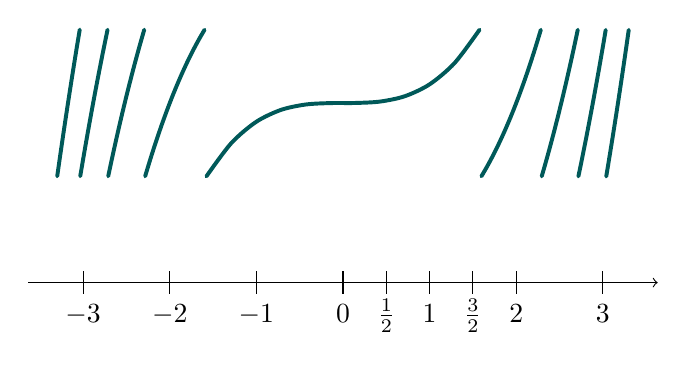
\begin{tikzpicture}[xscale=1.1,yscale=1.9,
     declare function={
         sdrob(\x) = Mod(\x+0.5, 1) - 0.5;
         main(\x) = (0.5 * \x)^3;
         invmain(\x) = \x^(1/3) * 2;}]

  \draw[->] ({invmain(-6)}, -1.2)
         -- ({invmain(6)}, -1.2);

  \foreach \x / \xtext in {0 / 0, -1 / -1,
    0.5 / \frac{1}{2}, 1.5 / \frac{3}{2},
    1 / 1, 2 / 2, 3 / 3, -2 / -2, -3 / -3}
   {\draw (\x cm,-11.25 mm) -- (\x cm,-12.75 mm)
      node[below, text height=1.6ex]{$\xtext$};}

  \foreach \t in {-4,...,4} {
    \draw[domain=invmain(\t-0.49):invmain(\t+0.49),
          variable=\x, samples=12, Cyan!35!black,
          line cap=round, line width=0.5mm,
          smooth] plot({\x}, {sdrob(main(\x))});
  }
\end{tikzpicture}
\end{tikzex-nobt}
